%kelompok 1 Sistem Operasi (Semaphore)
%Kelas D4 TI 1B
%Adam Noer Hidayatullah 1174097
%Ichsan Hizman
%Teddy
%Nisrina Aulia
%Irvan Rizkiansyah 1174043

\section{Komunikasi Serial pada Linux}
	
	\subsection{Konsep Dasar Komunikasi Serial}
	Suatu komunikasi yang dilakukan dimana suatu pengiriman data dilakukan per bit ialah dinamakan komunikasi serial, sehingga akan lebih lambat jika dibandingkan dengan komunikasi parallel seperti yang ada pada port printer yang dapat mengirim 8 bit sekaligus dalam sekali detak.
	Terdapat 2 macam cara komunikasi data serial yaitu :
		\begin{enumerate}
			\item Komunikasi data serial sinkron
			\item Komunikasi data serial asinkron
		\end{enumerate}
	
	Terdapat 2 kelompok device pada komunikasi serial yaitu :
		\begin{enumerate}
			\item Data Communication Equipment (DCE)
			Contohnya seperti scanner, printer, modem dan yang lainnya.
			\item Data Terminal Equipment (DTE)
			Contohnya sepertia terminal yang ada pada komputer.
		\end{enumerate}
	
	Keuntungan menggunakan port serial
		\begin{itemize}
			\item Masalah cable loss tidak akan menjadi suatu masalah yang besar pada komunikasi dengan kabel yang panjang, dari pada menggunakan kabel paralel. Port paralel akan mentransmisikan \"0\" pada tegangan 0 volt dan \"1\" di tegangan 1 volt, sedangkan port serial akan mentransmisikan \"1\" di tegangan -3 - -25 volt dan \"0\" di tegangan +3 - +25 volt.
			\item Hanya membutuhkan jumlah kabel yang sedikit, menggunakan 3 kabel saja pun bisa yaitu saluran Ground, saluran Transmit Data, saluran Receive Data.
			\item Populernya penggunaan mikrokontroler dan kebanyakan mikrokontroler dilengkapi dengan Serial Communication Interface (SCI) yang bisa dipaki untuk melakukan komunikasi dengan port serial pada komputer.
		\end{itemize}

	\subsection{Interprocess Communication}
	komunikasi antar proses untuk mengirim data dari satu proses ke proses yang lain, baik antar proses dalam satu komputer maupun proses dalam komputer yang berbeda
	karakteristik dari Interprocess Communincation yaitu:
		\begin{enumerate}
			\item komunikasi Synchronous dan asynchronous
				pada Sinkronisasi Synchronous, proses pengiriman dan penerimaan pada setiap pesan dan sistem ini akan berfungsi, jika sistem mengirim pesan, maka sistem hanya akan dapat merespon, sampai pesan selesai. Dalam komunikasi asynchronous, komunikasi ini dapat langsung memproses pesan, begitu pesan berada di buffer lokal, dan mengirim pesan dengan benar.
			\item Message destinations
					tempat tujuan dari sebuah pesan yang terdapat pada  sebuah computer adalah local port, yang didefinisikan berarti sebagai variable angka dengan tipe integer. Sebuah port pasti mempunyai satu penerima, akan tetapi bisa memiliki banyak pengirim.
			\item Reliability
					Keandalan suatu sistem dapat dilihat dari validitas dan integritas sistem.
					Sistem bila dilihat dari validitas, dapat dikatakan handal jika pesan yang disampaikan dijamin hingga tidak ada pesan yang hilang atau jatuh, dan sebaliknya.
			\item Ordering
				  menginginkan pesan yang terkirim dari pengirim dapat diterima sesuai dengan urutan grouping / ordering berdasarkan pesan awal yang terikirim.
		\end{enumerate}

	\subsection{Fungsi utama komunikasi serial}
		fungsi yang paling penting dari komunikasi serial pada mikrokontroler adalah untuk menyambungkan antara komputer dan mikrokontroler, dengan demikian kedua dapat bekerjasama.
	
	\subsection{contoh fungsi utama}
	contoh dari fungsi komunikasi serial seperti monitiring suhu menggunakan komputer, data suhu tersebut didapatkan oleh mikrokontroler lalu data tersebut ke komputer.
	
	\subsection{dua metode komunikasi serial}
	ada dua metode untuk komunikasi serial.
	pertama menggunakan port USB, metode ini disarankan karena USB terdapat pada PC yang dapat digunakan dimana saja pada usb port.
	kedua menggunakan menggunakan port serial, digunakan sebagai penghubung antara mikrokontroler dengan komputer PC.
	
	\subsection{macam-macam perintah terminal linux}
	macam macam perintah terminal pada linux:
		\begin{enumerate}
			\item cd (Change Directory) berguna untuk berpindah direktori. Sedangkan menggunakan perintah \"cd\" tanpa nama direktori akan mengantarkan anda kembali ke home direktori linux.
			\item rm files yaitu berguna untuk melakukan penghapusan sebuah file.
			\item mkdir berguna untuk membuat sebuah direktori yang baru, dengan membuat sebuah folder yang baru dengan menggunakan nama folder baru.
		\end{enumerate}
		
	\subsection{perbedaan port USB dan port serial}
	perbedaan port USB dengan port serial :
	perbedaannya adalah pada media penghubungannya, yaitu di port USB tidak bisa menggunakan rangkaian RS232 yang bisa digunakan sebagai media pengirim dan menerima data. Sedangkan pada metode port serial akan menggunakan sebuah rangkaian tambahan, yaitu sebuah rangkaian RS232 dan kabel serial yang digunakan sebagai penghubungnya.
	
	\subsection{cara menggunakan komukasi serial menggunakan port serial menjadi port USB}
	cara komunikasi serial menggunakan port serial diubah menjadi port USB yaitu menggunakan sebuah alat konverter yang dinamakan serial to USB conterver
	dan kabel USB male to male.
	
	\subsection{Koneksi Linux ke Serial Port}
	Untuk melakukan setting pada suatu perangkat, terkadang harus masuk terlebuh dahulu ke dalam console box. Biasanya akan menggunakan hyperterminal, namun software bawaan seperti itu tidak terdapat pada linux pada saat linux terinstall. Maka dari itu terdapat sebuah software yang dapat digunakan pada linux untuk melakukan komunikasi serial yaitu minicom untuk menggantikan hyperterminal.
	
	Software terminal minicom dapat di install dengan mudah di linux. Pertama buka terminal pada linux lalu ketik perintah :

	sudo apt-get install minicom

	Setelah itu software akan terinstall. Kemudian koneksikan ke perangkat yang akan digunakan menggunakan kabel console pada port serial. Lalu cek pada terminal linux dengan menggunakan perintah :

	dmesg | grep tty
	
	Perintah tersebut berguna untuk mengetahui port mana saja yang digunakan, seperti pada gambar dibawah ini
	
	\begin{figure} [ht]
	\centerline{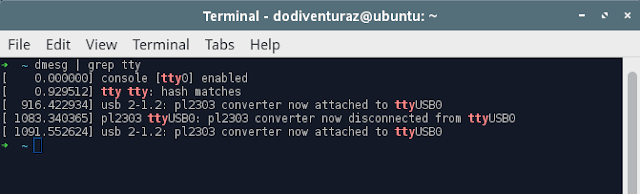
\includegraphics[width=1\textwidth]{figures/serialunix.png}}
	\caption{Gambar Status Serial}
	\label{statusserial}
	\end{figure}
	
	\ref{serialunix}
	
	Lalu ketikkan perintah :
	
	sudo minicom -s
	
	dan akan muncul seperti dibawah ini :
	
	\begin{table}[H]
		\begin{tabular}{|c|}
			\hline
			----configuration----\\
			\hline
			Filenames and paths\\
			\hline
			File transfer protocols\\
			\hline
			Serial port setup\\
			\hline
			Modem and dialing\\
			\hline
			Screen and keyboard\\
			\hline
			Save setup as dfl\\
			\hline
			Save setup as..\\
			\hline
			Exit\\
			\hline
			Exit from Minicom\\
		\end{tabular}
	\end{table}
	
	Kemudian pilih Serial Port Setup untuk mengetahui port yang terdeteksi, lalu akan muncul tampilan sebagai berikut :
	
	\begin{figure} [ht]
	\centerline{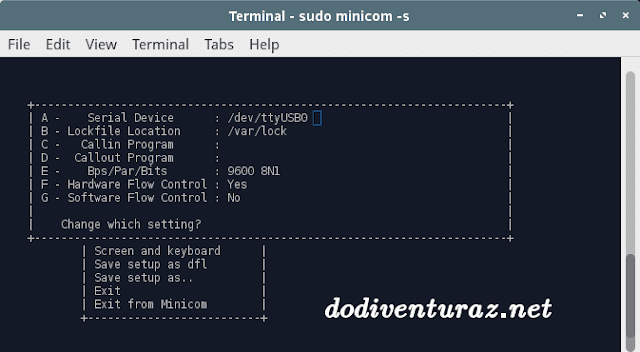
\includegraphics[width=1\textwidth]{figures/minicom.png}}
	\caption{Gambar minicom}
	\label{minicom}
	\end{figure}
	
	\ref{minicom}
	
	Lalu lakukan konfigurasi yang diperlukan sesuai kebutuhan yang diperlukan. Setelah konfigurasi selesai kembali ke menu utama dan pilih Save Setup as dfl. Kemudian pilih Exit, dan akan kembali ke terminal linux sebelumnya, kemudian ketikan perintah 
	
	\"minicom\"
	Maka Perangkat akan terkoneksi sesuai keinginan.

Dirangkum dari makalah \cite{fasnacht2008serial}
Dirangkum dari makalah \cite{barabanov1997linux}	


